\documentclass{report}
\usepackage{float}

\documentclass[12pt]{article}
\usepackage{array}
\usepackage{color}
\usepackage{amsthm}
\usepackage{eufrak}
\usepackage{lipsum}
\usepackage{pifont}
\usepackage{yfonts}
\usepackage{amsmath}
\usepackage{amssymb}
\usepackage{ccfonts}
\usepackage{comment} \usepackage{amsfonts}
\usepackage{fancyhdr}
\usepackage{graphicx}
\usepackage{listings}
\usepackage{mathrsfs}
\usepackage{setspace}
\usepackage{textcomp}
\usepackage{blindtext}
\usepackage{enumerate}
\usepackage{microtype}
\usepackage{xfakebold}
\usepackage{kantlipsum}
%\usepackage{draftwatermark}
\usepackage[spanish]{babel}
\usepackage[margin=1.5cm, top=2cm, bottom=2cm]{geometry}
\usepackage[framemethod=tikz]{mdframed}
\usepackage[colorlinks=true,citecolor=blue,linkcolor=red,urlcolor=magenta]{hyperref}

%//////////////////////////////////////////////////////
% Watermark configuration
%//////////////////////////////////////////////////////
%\SetWatermarkScale{4}
%\SetWatermarkColor{black}
%\SetWatermarkLightness{0.95}
%\SetWatermarkText{\texttt{Watermark}}

%//////////////////////////////////////////////////////
% Frame configuration
%//////////////////////////////////////////////////////
\newmdenv[tikzsetting={draw=gray,fill=white,fill opacity=0},backgroundcolor=none]{Frame}

%//////////////////////////////////////////////////////
% Font style configuration
%//////////////////////////////////////////////////////
\renewcommand{\familydefault}{\ttdefault}
\renewcommand{\rmdefault}{tt}

%//////////////////////////////////////////////////////
% Bold configuration
%//////////////////////////////////////////////////////
\newcommand{\fbseries}{\unskip\setBold\aftergroup\unsetBold\aftergroup\ignorespaces}
\makeatletter
\newcommand{\setBoldness}[1]{\def\fake@bold{#1}}
\makeatother

%//////////////////////////////////////////////////////
% Default font configuration
%//////////////////////////////////////////////////////
\DeclareFontFamily{\encodingdefault}{\ttdefault}{%
  \hyphenchar\font=\defaulthyphenchar
  \fontdimen2\font=0.33333em
  \fontdimen3\font=0.16667em
  \fontdimen4\font=0.11111em
  \fontdimen7\font=0.11111em}


%From M275 "Topology" at SJSU
\newcommand{\id}{\mathrm{id}}
\newcommand{\taking}[1]{\xrightarrow{#1}}
\newcommand{\inv}{^{-1}}

%From M170 "Introduction to Graph Theory" at SJSU
\DeclareMathOperator{\diam}{diam}
\DeclareMathOperator{\ord}{ord}
\newcommand{\defeq}{\overset{\mathrm{def}}{=}}

%From the USAMO .tex files
\newcommand{\ts}{\textsuperscript}
\newcommand{\dg}{^\circ}
\newcommand{\ii}{\item}

% % From Math 55 and Math 145 at Harvard
% \newenvironment{subproof}[1][Proof]{%
% \begin{proof}[#1] \renewcommand{\qedsymbol}{$\blacksquare$}}%
% {\end{proof}}

\newcommand{\liff}{\leftrightarrow}
\newcommand{\lthen}{\rightarrow}
\newcommand{\opname}{\operatorname}
\newcommand{\surjto}{\twoheadrightarrow}
\newcommand{\injto}{\hookrightarrow}
\newcommand{\On}{\mathrm{On}} % ordinals
\DeclareMathOperator{\img}{im} % Image
\DeclareMathOperator{\Img}{Im} % Image
\DeclareMathOperator{\coker}{coker} % Cokernel
\DeclareMathOperator{\Coker}{Coker} % Cokernel
\DeclareMathOperator{\Ker}{Ker} % Kernel
\DeclareMathOperator{\rank}{rank}
\DeclareMathOperator{\Spec}{Spec} % spectrum
\DeclareMathOperator{\Tr}{Tr} % trace
\DeclareMathOperator{\pr}{pr} % projection
\DeclareMathOperator{\ext}{ext} % extension
\DeclareMathOperator{\pred}{pred} % predecessor
\DeclareMathOperator{\dom}{dom} % domain
\DeclareMathOperator{\ran}{ran} % range
\DeclareMathOperator{\Hom}{Hom} % homomorphism
\DeclareMathOperator{\Mor}{Mor} % morphisms
\DeclareMathOperator{\End}{End} % endomorphism

\newcommand{\eps}{\epsilon}
\newcommand{\veps}{\varepsilon}
\newcommand{\ol}{\overline}
\newcommand{\ul}{\underline}
\newcommand{\wt}{\widetilde}
\newcommand{\wh}{\widehat}
\newcommand{\vocab}[1]{\textbf{\color{blue} #1}}
\providecommand{\half}{\frac{1}{2}}
\newcommand{\dang}{\measuredangle} %% Directed angle
\newcommand{\ray}[1]{\overrightarrow{#1}}
\newcommand{\seg}[1]{\overline{#1}}
\newcommand{\arc}[1]{\wideparen{#1}}
\DeclareMathOperator{\cis}{cis}
\DeclareMathOperator*{\lcm}{lcm}
\DeclareMathOperator*{\argmin}{arg min}
\DeclareMathOperator*{\argmax}{arg max}
\newcommand{\cycsum}{\sum_{\mathrm{cyc}}}
\newcommand{\symsum}{\sum_{\mathrm{sym}}}
\newcommand{\cycprod}{\prod_{\mathrm{cyc}}}
\newcommand{\symprod}{\prod_{\mathrm{sym}}}
\newcommand{\Qed}{\begin{flushright}\qed\end{flushright}}
\newcommand{\parinn}{\setlength{\parindent}{1cm}}
\newcommand{\parinf}{\setlength{\parindent}{0cm}}
% \newcommand{\norm}{\|\cdot\|}
\newcommand{\inorm}{\norm_{\infty}}
\newcommand{\opensets}{\{V_{\alpha}\}_{\alpha\in I}}
\newcommand{\oset}{V_{\alpha}}
\newcommand{\opset}[1]{V_{\alpha_{#1}}}
\newcommand{\lub}{\text{lub}}
\newcommand{\del}[2]{\frac{\partial #1}{\partial #2}}
\newcommand{\Del}[3]{\frac{\partial^{#1} #2}{\partial^{#1} #3}}
\newcommand{\deld}[2]{\dfrac{\partial #1}{\partial #2}}
\newcommand{\Deld}[3]{\dfrac{\partial^{#1} #2}{\partial^{#1} #3}}
\newcommand{\lm}{\lambda}
\newcommand{\uin}{\mathbin{\rotatebox[origin=c]{90}{$\in$}}}
\newcommand{\usubset}{\mathbin{\rotatebox[origin=c]{90}{$\subset$}}}
\newcommand{\lt}{\left}
\newcommand{\rt}{\right}
\newcommand{\paren}[1]{\left(#1\right)}
\newcommand{\bs}[1]{\boldsymbol{#1}}
\newcommand{\exs}{\exists}
\newcommand{\st}{\strut}
\newcommand{\dps}[1]{\displaystyle{#1}}

\newcommand{\sol}{\setlength{\parindent}{0cm}\textbf{\textit{Solution:}}\setlength{\parindent}{1cm} }
\newcommand{\solve}[1]{\setlength{\parindent}{0cm}\textbf{\textit{Solution: }}\setlength{\parindent}{1cm}#1 \Qed}

% Things Lie
\newcommand{\kb}{\mathfrak b}
\newcommand{\kg}{\mathfrak g}
\newcommand{\kh}{\mathfrak h}
\newcommand{\kn}{\mathfrak n}
\newcommand{\ku}{\mathfrak u}
\newcommand{\kz}{\mathfrak z}
\DeclareMathOperator{\Ext}{Ext} % Ext functor
\DeclareMathOperator{\Tor}{Tor} % Tor functor
\newcommand{\gl}{\opname{\mathfrak{gl}}} % frak gl group
\renewcommand{\sl}{\opname{\mathfrak{sl}}} % frak sl group chktex 6

% More script letters etc.
\newcommand{\SA}{\mathcal A}
\newcommand{\SB}{\mathcal B}
\newcommand{\SC}{\mathcal C}
\newcommand{\SF}{\mathcal F}
\newcommand{\SG}{\mathcal G}
\newcommand{\SH}{\mathcal H}
\newcommand{\OO}{\mathcal O}

\newcommand{\SCA}{\mathscr A}
\newcommand{\SCB}{\mathscr B}
\newcommand{\SCC}{\mathscr C}
\newcommand{\SCD}{\mathscr D}
\newcommand{\SCE}{\mathscr E}
\newcommand{\SCF}{\mathscr F}
\newcommand{\SCG}{\mathscr G}
\newcommand{\SCH}{\mathscr H}

% Mathfrak primes
\newcommand{\km}{\mathfrak m}
\newcommand{\kp}{\mathfrak p}
\newcommand{\kq}{\mathfrak q}

% number sets
\newcommand{\RR}[1][]{\ensuremath{\ifstrempty{#1}{\mathbb{R}}{\mathbb{R}^{#1}}}}
\newcommand{\NN}[1][]{\ensuremath{\ifstrempty{#1}{\mathbb{N}}{\mathbb{N}^{#1}}}}
\newcommand{\ZZ}[1][]{\ensuremath{\ifstrempty{#1}{\mathbb{Z}}{\mathbb{Z}^{#1}}}}
\newcommand{\QQ}[1][]{\ensuremath{\ifstrempty{#1}{\mathbb{Q}}{\mathbb{Q}^{#1}}}}
\newcommand{\CC}[1][]{\ensuremath{\ifstrempty{#1}{\mathbb{C}}{\mathbb{C}^{#1}}}}
\newcommand{\PP}[1][]{\ensuremath{\ifstrempty{#1}{\mathbb{P}}{\mathbb{P}^{#1}}}}
\newcommand{\HH}[1][]{\ensuremath{\ifstrempty{#1}{\mathbb{H}}{\mathbb{H}^{#1}}}}
\newcommand{\FF}[1][]{\ensuremath{\ifstrempty{#1}{\mathbb{F}}{\mathbb{F}^{#1}}}}
% expected value
\newcommand{\EE}{\ensuremath{\mathbb{E}}}
\newcommand{\charin}{\text{ char }}
\DeclareMathOperator{\sign}{sign}
\DeclareMathOperator{\Aut}{Aut}
\DeclareMathOperator{\Inn}{Inn}
\DeclareMathOperator{\Syl}{Syl}
\DeclareMathOperator{\Gal}{Gal}
\DeclareMathOperator{\GL}{GL} % General linear group
\DeclareMathOperator{\SL}{SL} % Special linear group

%---------------------------------------
% BlackBoard Math Fonts :-
%---------------------------------------

%Captital Letters
\newcommand{\bbA}{\mathbb{A}}	\newcommand{\bbB}{\mathbb{B}}
\newcommand{\bbC}{\mathbb{C}}	\newcommand{\bbD}{\mathbb{D}}
\newcommand{\bbE}{\mathbb{E}}	\newcommand{\bbF}{\mathbb{F}}
\newcommand{\bbG}{\mathbb{G}}	\newcommand{\bbH}{\mathbb{H}}
\newcommand{\bbI}{\mathbb{I}}	\newcommand{\bbJ}{\mathbb{J}}
\newcommand{\bbK}{\mathbb{K}}	\newcommand{\bbL}{\mathbb{L}}
\newcommand{\bbM}{\mathbb{M}}	\newcommand{\bbN}{\mathbb{N}}
\newcommand{\bbO}{\mathbb{O}}	\newcommand{\bbP}{\mathbb{P}}
\newcommand{\bbQ}{\mathbb{Q}}	\newcommand{\bbR}{\mathbb{R}}
\newcommand{\bbS}{\mathbb{S}}	\newcommand{\bbT}{\mathbb{T}}
\newcommand{\bbU}{\mathbb{U}}	\newcommand{\bbV}{\mathbb{V}}
\newcommand{\bbW}{\mathbb{W}}	\newcommand{\bbX}{\mathbb{X}}
\newcommand{\bbY}{\mathbb{Y}}	\newcommand{\bbZ}{\mathbb{Z}}

%---------------------------------------
% MathCal Fonts :-
%---------------------------------------

%Captital Letters
\newcommand{\mcA}{\mathcal{A}}	\newcommand{\mcB}{\mathcal{B}}
\newcommand{\mcC}{\mathcal{C}}	\newcommand{\mcD}{\mathcal{D}}
\newcommand{\mcE}{\mathcal{E}}	\newcommand{\mcF}{\mathcal{F}}
\newcommand{\mcG}{\mathcal{G}}	\newcommand{\mcH}{\mathcal{H}}
\newcommand{\mcI}{\mathcal{I}}	\newcommand{\mcJ}{\mathcal{J}}
\newcommand{\mcK}{\mathcal{K}}	\newcommand{\mcL}{\mathcal{L}}
\newcommand{\mcM}{\mathcal{M}}	\newcommand{\mcN}{\mathcal{N}}
\newcommand{\mcO}{\mathcal{O}}	\newcommand{\mcP}{\mathcal{P}}
\newcommand{\mcQ}{\mathcal{Q}}	\newcommand{\mcR}{\mathcal{R}}
\newcommand{\mcS}{\mathcal{S}}	\newcommand{\mcT}{\mathcal{T}}
\newcommand{\mcU}{\mathcal{U}}	\newcommand{\mcV}{\mathcal{V}}
\newcommand{\mcW}{\mathcal{W}}	\newcommand{\mcX}{\mathcal{X}}
\newcommand{\mcY}{\mathcal{Y}}	\newcommand{\mcZ}{\mathcal{Z}}


%---------------------------------------
% Bold Math Fonts :-
%---------------------------------------

%Captital Letters
\newcommand{\bmA}{\boldsymbol{A}}	\newcommand{\bmB}{\boldsymbol{B}}
\newcommand{\bmC}{\boldsymbol{C}}	\newcommand{\bmD}{\boldsymbol{D}}
\newcommand{\bmE}{\boldsymbol{E}}	\newcommand{\bmF}{\boldsymbol{F}}
\newcommand{\bmG}{\boldsymbol{G}}	\newcommand{\bmH}{\boldsymbol{H}}
\newcommand{\bmI}{\boldsymbol{I}}	\newcommand{\bmJ}{\boldsymbol{J}}
\newcommand{\bmK}{\boldsymbol{K}}	\newcommand{\bmL}{\boldsymbol{L}}
\newcommand{\bmM}{\boldsymbol{M}}	\newcommand{\bmN}{\boldsymbol{N}}
\newcommand{\bmO}{\boldsymbol{O}}	\newcommand{\bmP}{\boldsymbol{P}}
\newcommand{\bmQ}{\boldsymbol{Q}}	\newcommand{\bmR}{\boldsymbol{R}}
\newcommand{\bmS}{\boldsymbol{S}}	\newcommand{\bmT}{\boldsymbol{T}}
\newcommand{\bmU}{\boldsymbol{U}}	\newcommand{\bmV}{\boldsymbol{V}}
\newcommand{\bmW}{\boldsymbol{W}}	\newcommand{\bmX}{\boldsymbol{X}}
\newcommand{\bmY}{\boldsymbol{Y}}	\newcommand{\bmZ}{\boldsymbol{Z}}
%Small Letters
\newcommand{\bma}{\boldsymbol{a}}	\newcommand{\bmb}{\boldsymbol{b}}
\newcommand{\bmc}{\boldsymbol{c}}	\newcommand{\bmd}{\boldsymbol{d}}
\newcommand{\bme}{\boldsymbol{e}}	\newcommand{\bmf}{\boldsymbol{f}}
\newcommand{\bmg}{\boldsymbol{g}}	\newcommand{\bmh}{\boldsymbol{h}}
\newcommand{\bmi}{\boldsymbol{i}}	\newcommand{\bmj}{\boldsymbol{j}}
\newcommand{\bmk}{\boldsymbol{k}}	\newcommand{\bml}{\boldsymbol{l}}
\newcommand{\bmm}{\boldsymbol{m}}	\newcommand{\bmn}{\boldsymbol{n}}
\newcommand{\bmo}{\boldsymbol{o}}	\newcommand{\bmp}{\boldsymbol{p}}
\newcommand{\bmq}{\boldsymbol{q}}	\newcommand{\bmr}{\boldsymbol{r}}
\newcommand{\bms}{\boldsymbol{s}}	\newcommand{\bmt}{\boldsymbol{t}}
\newcommand{\bmu}{\boldsymbol{u}}	\newcommand{\bmv}{\boldsymbol{v}}
\newcommand{\bmw}{\boldsymbol{w}}	\newcommand{\bmx}{\boldsymbol{x}}
\newcommand{\bmy}{\boldsymbol{y}}	\newcommand{\bmz}{\boldsymbol{z}}

%---------------------------------------
% Scr Math Fonts :-
%---------------------------------------

\newcommand{\sA}{{\mathscr{A}}}   \newcommand{\sB}{{\mathscr{B}}}
\newcommand{\sC}{{\mathscr{C}}}   \newcommand{\sD}{{\mathscr{D}}}
\newcommand{\sE}{{\mathscr{E}}}   \newcommand{\sF}{{\mathscr{F}}}
\newcommand{\sG}{{\mathscr{G}}}   \newcommand{\sH}{{\mathscr{H}}}
\newcommand{\sI}{{\mathscr{I}}}   \newcommand{\sJ}{{\mathscr{J}}}
\newcommand{\sK}{{\mathscr{K}}}   \newcommand{\sL}{{\mathscr{L}}}
\newcommand{\sM}{{\mathscr{M}}}   \newcommand{\sN}{{\mathscr{N}}}
\newcommand{\sO}{{\mathscr{O}}}   \newcommand{\sP}{{\mathscr{P}}}
\newcommand{\sQ}{{\mathscr{Q}}}   \newcommand{\sR}{{\mathscr{R}}}
\newcommand{\sS}{{\mathscr{S}}}   \newcommand{\sT}{{\mathscr{T}}}
\newcommand{\sU}{{\mathscr{U}}}   \newcommand{\sV}{{\mathscr{V}}}
\newcommand{\sW}{{\mathscr{W}}}   \newcommand{\sX}{{\mathscr{X}}}
\newcommand{\sY}{{\mathscr{Y}}}   \newcommand{\sZ}{{\mathscr{Z}}}


%---------------------------------------
% Math Fraktur Font
%---------------------------------------

%Captital Letters
\newcommand{\mfA}{\mathfrak{A}}	\newcommand{\mfB}{\mathfrak{B}}
\newcommand{\mfC}{\mathfrak{C}}	\newcommand{\mfD}{\mathfrak{D}}
\newcommand{\mfE}{\mathfrak{E}}	\newcommand{\mfF}{\mathfrak{F}}
\newcommand{\mfG}{\mathfrak{G}}	\newcommand{\mfH}{\mathfrak{H}}
\newcommand{\mfI}{\mathfrak{I}}	\newcommand{\mfJ}{\mathfrak{J}}
\newcommand{\mfK}{\mathfrak{K}}	\newcommand{\mfL}{\mathfrak{L}}
\newcommand{\mfM}{\mathfrak{M}}	\newcommand{\mfN}{\mathfrak{N}}
\newcommand{\mfO}{\mathfrak{O}}	\newcommand{\mfP}{\mathfrak{P}}
\newcommand{\mfQ}{\mathfrak{Q}}	\newcommand{\mfR}{\mathfrak{R}}
\newcommand{\mfS}{\mathfrak{S}}	\newcommand{\mfT}{\mathfrak{T}}
\newcommand{\mfU}{\mathfrak{U}}	\newcommand{\mfV}{\mathfrak{V}}
\newcommand{\mfW}{\mathfrak{W}}	\newcommand{\mfX}{\mathfrak{X}}
\newcommand{\mfY}{\mathfrak{Y}}	\newcommand{\mfZ}{\mathfrak{Z}}
%Small Letters
\newcommand{\mfa}{\mathfrak{a}}	\newcommand{\mfb}{\mathfrak{b}}
\newcommand{\mfc}{\mathfrak{c}}	\newcommand{\mfd}{\mathfrak{d}}
\newcommand{\mfe}{\mathfrak{e}}	\newcommand{\mff}{\mathfrak{f}}
\newcommand{\mfg}{\mathfrak{g}}	\newcommand{\mfh}{\mathfrak{h}}
\newcommand{\mfi}{\mathfrak{i}}	\newcommand{\mfj}{\mathfrak{j}}
\newcommand{\mfk}{\mathfrak{k}}	\newcommand{\mfl}{\mathfrak{l}}
\newcommand{\mfm}{\mathfrak{m}}	\newcommand{\mfn}{\mathfrak{n}}
\newcommand{\mfo}{\mathfrak{o}}	\newcommand{\mfp}{\mathfrak{p}}
\newcommand{\mfq}{\mathfrak{q}}	\newcommand{\mfr}{\mathfrak{r}}
\newcommand{\mfs}{\mathfrak{s}}	\newcommand{\mft}{\mathfrak{t}}
\newcommand{\mfu}{\mathfrak{u}}	\newcommand{\mfv}{\mathfrak{v}}
\newcommand{\mfw}{\mathfrak{w}}	\newcommand{\mfx}{\mathfrak{x}}
\newcommand{\mfy}{\mathfrak{y}}	\newcommand{\mfz}{\mathfrak{z}}


\title{\Huge{Métodos Matemático}\\Primera Tarea}
\author{\huge{Sergio Montoya}}
\date{}

\begin{document}

\maketitle
\newpage% or \cleardoublepage
% \pdfbookmark[<level>]{<title>}{<dest>}
\pdfbookmark[section]{\contentsname}{toc}
\tableofcontents
\pagebreak

\chapter{Primera Pregunta 11.2.3}
\label{chap:1}
\qs{11.2.3}{Encuentre la función analítica: \[
w\left( z \right) = u\left( x, y \right) + i v\left( x, y \right) 
.\] para 
\begin{itemize}
  \item $u\left( x, y \right) = x^{3} - 3xy^2$
  \item $v\left( x, y \right) = e^{-y}\sin\left( x \right) $
\end{itemize}}

\textbf{Solución: }
\begin{itemize}
  \item $u\left( x, y \right) = x^3 - 3xy^2$

    Recordemos las condiciones de Cauchy-Riemann \[
    \frac{\partial u}{\partial x} = \frac{\partial v}{\partial y} ; \frac{\partial u}{\partial y} = - \frac{\partial v}{\partial x} 
    .\] Con esto entonces partimos de $u\left( x, y \right) $ y debemos llegar a un $v\left( x, y \right) $ que permita cumplir las ecuaciones de Cauchy-Riemann.
    \begin{align*}
      \frac{\partial u}{\partial x} &= 3x^2 - 3y^2 = \frac{\partial v}{\partial y} \\
      v &= \int	3x^2 - 3y^2 dy\\
      &= 3x^2y - y^{3} + f\left( x \right) \\
      \frac{\partial u}{\partial y} &= -6xy\\
      \frac{\partial v}{\partial x} &= -\frac{\partial u}{\partial y} = 6xy \\
      \frac{\partial v}{\partial x} &= 6xy \\
      \implies c &= 0
    .\end{align*}
    
    Por lo tanto la función es:
    \begin{align*}
      u\left( x, y \right) &= x^3 - 3xy^2\\
      v\left( x, y \right) &= 3x^2y - y^{3} \\
      w\left( z \right) &= u\left( x, y \right) + v\left( x, y \right)  \\
      &= \left( x^3 - 3xy^2 \right) + i\left( 3x^2y - y^{3} \right)
    .\end{align*}

  \item $v\left( x, y \right) = e^{-y}\sin\left( x \right) $


    Recordemos las condiciones de Cauchy-Riemann \[
    \frac{\partial u}{\partial x} = \frac{\partial v}{\partial y} ; \frac{\partial u}{\partial y} = - \frac{\partial v}{\partial x} 
    .\] Con esto entonces partimos de $u\left( x, y \right) $ y debemos llegar a un $v\left( x, y \right) $ que permita cumplir las ecuaciones de Cauchy-Riemann.

    \begin{align*}
      \frac{\partial v}{\partial x} &= e^{-y}\cos\left( x \right) \\
      \frac{\partial u}{\partial y} &= - \frac{\partial v}{\partial x} = -e^{-y}\cos\left( x \right)  \\
      u &= \int -e^{-y}\cos\left( x \right) dy \\
      &= e^{-y}\cos\left( x \right) + f\left( x \right)  \\
      \frac{\partial v}{\partial y} &= -e^{-y}\sin\left( x \right)  \\
      \frac{\partial u}{\partial x} &= \frac{\partial v}{\partial y} = -e^{-y}\sin\left( x \right) \\
      \frac{\partial u}{\partial x} &= - e^{-y}\sin\left( x \right) + \dot{f\left( x \right) }\\
      f\left( x \right) &= 0 \\
    .\end{align*}

    Por lo tanto esto queda como
    \begin{align*}
      u\left( x, y \right) &= e^{-y}\cos\left( x \right) \\
      v\left( x, y \right) &= e^{-y}\sin\left( x \right) \\
      w\left( z \right) &= e^{-y}\cos\left( x \right) + e^{-y}\sin\left( x \right)
    .\end{align*}
\end{itemize}

\chapter{Segunda Pregunta 11.2.11}
\label{chap:2}

\qs{11.2.11}{
Un flujo en un fluido dos dimensional es descrito por potencial complejo $f\left( z \right) = u\left( x, v \right) + iv\left( x, y \right) $. La velocidad del fluido $V$ esta dada por $V = \nabla u$. Si $f\left( z \right) $es analítica entonces: 
\begin{itemize}
  \item Muestre que $ \frac{df}{dz} = V_x - i V_y$
  \item Muestre que $\nabla \cdot V = 0$ 
  \item Muestre que $\nabla \times V = 0$
\end{itemize}
}
\begin{itemize}
  \item Para comenzar tenemos por el capitulo previo que: \[
  \frac{df}{dz} = \frac{\partial u}{\partial x} + i \frac{\partial v}{\partial x} 
  .\] Sin embargo, por las ecuaciones de Cauchy-Riemann tenemos que \[
  \frac{\partial v}{\partial x} = - \frac{\partial u}{\partial y} 
  .\] Por lo cual esta ecuación queda como: \[
  \frac{df}{dz} = \frac{\partial u}{\partial x} - i \frac{\partial u}{\partial y} 
  .\] Recordemos ahora que $V = \nabla u = \left< \frac{\partial u}{\partial x} , \frac{\partial u}{\partial y} , \frac{\partial u}{\partial z} \right>$ por lo tanto se puede resumir como \[
  \frac{df}{dz} = V_x - i V_y
  .\] 
  \nt{Se que en este caso $\frac{\partial u}{\partial z} $ no tiene sentido. Por lo tanto este sera igual a $0$ sin embargo esta sera la notación que voy a mantener dado que en el ultimo punto tenemos que hacer producto cruz que existe en solamente en $3$ dimensiones. Mientras tanto esto es simplemente una proyección de tres dimensiones a dos. Específicamente al plano $z = 0$
  }
  \item Tomemos \[
      V = \nabla u = \left< \frac{\partial u}{\partial x} , \frac{\partial u}{\partial y} , \frac{\partial u}{\partial z} \right>
  .\] Sin embargo, aprovechémonos de las ecuaciones de Cauchy-Riemann  por lo que \[
  V = \nabla u = \left<\frac{\partial v}{\partial y} , - \frac{\partial v}{\partial x} , \frac{\partial u}{\partial z}  \right>
  .\] Por lo tanto ahora podemos desarrollar y quedaría:
  \begin{align*}
    \nabla \cdot \nabla u &= \frac{\partial^2 v}{\partial x\partial y} - \frac{\partial^2 v}{\partial y \partial x} + \frac{\partial^2 u}{\partial z^2}   \\
			  &= \cancel{\frac{\partial^2 v}{\partial x\partial y}} - \cancel{\frac{\partial^2 v}{\partial y \partial x}} + 0\\
			  &= 0
.\end{align*} Recordemos que las segundas derivadas son simétricas en este caso por el \textit{Teorema de Shwarz}
  \item Para esto no tenemos que hacer realmente ningún ajuste. Recordemos entonces que 
    \begin{align*}
      \nabla \times \nabla u &= det \left(\begin{pmatrix} 
    \hat{i}& \hat{j} & \hat{k}\\
    \frac{\partial }{\partial x} & \frac{\partial }{\partial y} & \frac{\partial }{\partial z} \\
    \frac{\partial u}{\partial x} & \frac{\partial u}{\partial y} & \frac{\partial u}{\partial z} 
  \end{pmatrix} \right)\\
			     &= \hat{i}\left( \frac{\partial^2 u}{\partial y\partial z} - \frac{\partial^2 u}{\partial y\partial z}  \right) \\ 
			     &\ - \hat{j}\left( \frac{\partial^2 u}{\partial x\partial z} - \frac{\partial^2 u}{\partial x\partial z}  \right) \\ 
			     &\ + \hat{k}\left( \frac{\partial^2 u}{\partial x \partial y} - \frac{\partial u}{\partial x \partial y}  \right)   \\
  &= 0 \hat{i} + 0 \hat{j} + 0 \hat{k} \\
  &= 0 \\
\end{align*}
\end{itemize}

\chapter{Tercera Pregunta 11.4.3}
\label{chap:3}

\qs{11.4.3}{
Asumiendo que $f\left( z \right) $ es analítica en un contorno cerrado $C$ y que el punto $z_0$ esta dentro de $C$, muestre que: \[
  \oint_C \frac{f'\left( z \right) }{z - z_0}dz = \oint_C \frac{f\left( z \right) }{\left( z - z_0 \right)^2}dz
.\] 
}

Partamos de la formula de Cauchy: \[
\frac{1}{2\pi i}\oint_C \frac{f\left( z \right) }{z - z_0} dz = f\left( z_0 \right) 
.\] Note que podemos definir una función: \[
F\left( z_0 \right) = \frac{1}{2\pi i}\oint_C \frac{f\left( z \right) }{z - z_0} = f\left( z_0 \right) 
.\] por lo tanto podemos derivar con respecto a $z_0$ lo que entonces nos permite desarrollar:
\begin{align*}
  \frac{d}{dz_0}\left( \frac{1}{2\pi i}\oint_C \frac{f\left( z \right) }{z - z_0}dz\right) &= f'\left( z_0 \right)\\
  \frac{1}{2\pi i}\oint_C \frac{d}{dz_0}\left( \frac{f\left( z \right) }{z - z_0} \right) dz &= f'\left( z_0 \right)  \\
  \frac{1}{2\pi i}\oint_C \frac{f\left( z \right) }{\left( z - z_0 \right)^{2} }dz &= f'\left( z_0 \right)
.\end{align*}

Ahora partiendo desde el otro lado, notemos que 
\begin{align*}
  \oint_C \frac{f'\left( z \right) }{z - z_0}dz &= 2\pi i f'\left( z_0 \right) \\
  f'\left( z_0 \right) &= \frac{1}{2\pi i}\oint_C \frac{f\left( z \right) }{\left( z - z_0 \right)^{2} }dz  \\
  \oint_C \frac{f'\left( z \right) }{z - z_0}dz &= 2\pi i\frac{1}{2\pi i}\oint_C \frac{f\left( z \right) }{\left( z - z_0 \right)^{2} }dz  \\
  \oint_C \frac{f'\left( z \right) }{z - z_0}dz &= \oint_C \frac{f\left( z \right) }{\left( z - z_0 \right)^2}dz
.\end{align*}

\chapter{Cuarta Pregunta 11.4.9}
\label{chap:4}

\qs{11.4.9}{
  Evalué \[
    \oint_{C} \frac{f\left( z \right) }{z\left( 2z + 1 \right)^2} 
  \] Para el contorno del circulo unitario

  \textit{Pista:} Haga expansión de fracciones parciales.
}

Para comenzar sigamos la pista de hacer una expansión de fracciones parciales. Esto nos indica que 
\begin{align*}
  \frac{1}{z\left( 2z + 1 \right)^2} &= \frac{A}{z} + \frac{B}{2z + 1} + \frac{C}{ \left( 2z + 1 \right)^2} \\
  \frac{\cancel{z}}{\cancel{z}\left( 2z + 1 \right)^2} &= A + \frac{zB}{2z + 1} + \frac{zC}{\left( 2z + 1 \right)^2};\ z = 0 \\
  1 &= A \\
\frac{\cancel{\left( 2z + 1 \right)^2}}{z \cancel{\left( 2z + 1 \right)^2}} &= \frac{\left( 2z + 1 \right)^2}{z} + \left( 2z + 1 \right) B + C;\ z = -\frac{1}{2}\\
-2 &= C \\
\frac{1}{z\left( 2z + 1 \right)^2} &= \frac{1}{z} + \frac{B}{2z + 1} - \frac{2}{\left( 2z + 1 \right)^2};\ z = -1 \\
-1 &= -1 - B - 2\\
B &= -2 \\
\frac{1}{z\left( 2z + 1 \right) } &= \frac{1}{z} - \frac{2}{2z + 1} - \frac{2}{\left( 2z + 1 \right)^2} \\
.\end{align*}

Por lo tanto esta misma integral nos queda como: \[
    \oint_{C} \frac{f\left( z \right) }{z\left( 2z + 1 \right)^2} =
\oint_{C} \frac{f\left( z \right) }{z} dz - 2\oint_{C} \frac{f\left( z \right) }{2\left( 1 + \frac{1}{2} \right) }dz - 2 \oint_{C} \frac{f\left( z \right) }{4\left( 1 + \frac{1}{2} \right)^2} dz
.\] Que reduciendo y apoyándonos en el capitulo \ref{chap:3} queda: \[
    \oint_{C} \frac{f\left( z \right) }{z\left( 2z + 1 \right)^2} =
\oint_{C} \frac{f\left( z \right) }{z} dz - \oint_{C} \frac{f\left( z \right) }{\left( 1 + \frac{1}{2} \right) }dz - \pi i f'\left( \frac{1}{2} \right) 
.\] Ahora podemos simplemente aplicar la formula de Cauchy y nos queda:
\begin{align*}
  \oint_{C} \frac{f\left( z \right) }{z\left( 2z + 1 \right)^2} &= 2\pi i f\left( 0 \right) - 2\pi i f\left( \frac{1}{2} \right) - \pi i f'\left( \frac{1}{2} \right)  \\ 
  &= 2\pi i\left( f\left( 0 \right) - f\left( \frac{1}{2} \right) - \frac{1}{2}f'\left( \frac{1}{2} \right)  \right) 
.\end{align*}

\chapter{Quinta Pregunta 11.6.6}
\label{chap:6}

\qs{11.6.6}{
  La función $F\left( z \right) = \ln\left( z^2 + 1 \right) $ esta hecho de un solo valor por una linea recta en cortes de rama de $\left( x, y \right) = \left( 0, -1 \right) $ a $\left( -\infty, -1 \right) $ y desde $\left( 0, +1 \right) $ a $\left( 0, +\infty \right) $. Vea la figura \ref{img:ayuda1}. Si $F\left( 0 \right) = -2\pi i$, encuentre el valor de $F\left( i - 2 \right) $ 

  \begin{figure}[H]
    \centering
    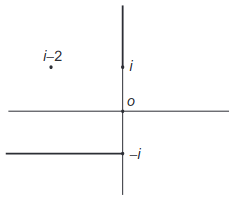
\includegraphics[width=0.3\textwidth]{img/ayuda.png}
    \caption{Cortes para el ejercicio del capitulo \ref{chap:6}}
    \label{img:ayuda1}
  \end{figure}
}

Iniciemos esta pregunta por ver en que rama de la función logaritmo estamos. Sabemos que $f\left( 0 \right) = -2\pi i $ Por lo tanto podemos desarrollar como:
\begin{align*}
  f\left( 0 \right) &= \ln\left( 0^2 + 1 \right)  \\
  &= \ln\left( 1 \right)  \\
  &= 0 + i \left( 0 + 2\pi n \right)  \\
  &= i 2\pi n  \\
  -i 2 \pi &= i 2\pi n \\
  n &= -1
.\end{align*}

Ahora con esto sabemos que la rama en la que nos encontramos es la rama $n = -1$. Ahora bien, por otro lado veamos el resultado de la función interna para el punto solicitado.
 \begin{align*}
  \left( i - 2 \right)^2 + 1 &= 3 - 4i + 1 \\
  &= 4 - 4i
.\end{align*}

Por lo tanto, estamos simplemente buscando el $\ln\left( 4 - 4i \right) $. Por un lado note que podemos sacar \[\left| 4 - 4i \right| = \sqrt{4^2 + 4^2} = \sqrt{4^2\left( 2 \right) } = 4\sqrt{2} \]. Por lo tanto ya tenemos la primera parte como $\ln\left( 4\sqrt{2}  \right) $. 

Ahora bien, para el angulo notemos que podemos evitar pasar por cualquier corte si tomamos valores de angulo negativo. En este caso podemos notar que el punto deseado esta justo en la mitad del cuadril 4. Por lo tanto tiene un angulo de $-\frac{\pi}{4}$ y como estamos en la rama $n = -1$ el resultado total es: \[
f\left( i - 2 \right) = \ln\left( 4 - 4i \right) = \ln\left( 4\sqrt{2}  \right) + i \left( -\frac{\pi}{4} - 2\pi \right) = \ln\left( 4\sqrt{2}  \right) - i \left( \frac{9\pi}{4} \right) 
.\] 

\end{document}
